%%%%%%%%%%%%%%%%%%%%%%%%%%%%%%%%%%%%%%%%%
% Jacobs Landscape Poster
% LaTeX Template
% Version 1.0 (29/03/13)
%
% Created by:
% Computational Physics and Biophysics Group, Jacobs University
% https://teamwork.jacobs-university.de:8443/confluence/display/CoPandBiG/LaTeX+Poster
% 
% Further modified by:
% Nathaniel Johnston (nathaniel@njohnston.ca)
%
% This template has been downloaded from:
% http://www.LaTeXTemplates.com
%
% License:
% CC BY-NC-SA 3.0 (http://creativecommons.org/licenses/by-nc-sa/3.0/)
%
%%%%%%%%%%%%%%%%%%%%%%%%%%%%%%%%%%%%%%%%%

%----------------------------------------------------------------------------------------
%	PACKAGES AND OTHER DOCUMENT CONFIGURATIONS
%----------------------------------------------------------------------------------------
\documentclass[final]{beamer}
 



\usepackage[scale=1.24]{beamerposter} % Use the beamerposter package for laying out the poster

\usetheme{confposter} % Use the confposter theme supplied with this template

\setbeamercolor{block title}{fg=ngreen,bg=white} % Colors of the block titles
\setbeamercolor{block body}{fg=black,bg=white} % Colors of the body of blocks
\setbeamercolor{block alerted title}{fg=white,bg=dblue!70} % Colors of the highlighted block titles
\setbeamercolor{block alerted body}{fg=black,bg=dblue!10} % Colors of the body of highlighted blocks
% Many more colors are available for use in beamerthemeconfposter.sty

%-----------------------------------------------------------
% Define the column widths and overall poster size
% To set effective sepwid, onecolwid and twocolwid values, first choose how many columns you want and how much separation you want between columns
% In this template, the separation width chosen is 0.024 of the paper width and a 4-column layout
% onecolwid should therefore be (1-(# of columns+1)*sepwid)/# of columns e.g. (1-(4+1)*0.024)/4 = 0.22
% Set twocolwid to be (2*onecolwid)+sepwid = 0.464
% Set threecolwid to be (3*onecolwid)+2*sepwid = 0.708

\newlength{\sepwid}
\newlength{\onecolwid}
\newlength{\twocolwid}
\newlength{\threecolwid}
\setlength{\paperwidth}{48in} % A0 width: 46.8in
\setlength{\paperheight}{36in} % A0 height: 33.1in
\setlength{\sepwid}{0.024\paperwidth} % Separation width (white space) between columns
\setlength{\onecolwid}{0.22\paperwidth} % Width of one column
\setlength{\twocolwid}{0.464\paperwidth} % Width of two columns
\setlength{\threecolwid}{0.708\paperwidth} % Width of three columns
\setlength{\topmargin}{-0.5in} % Reduce the top margin size
%-----------------------------------------------------------

\usepackage{graphicx}  % Required for including images

\usepackage{booktabs} % Top and bottom rules for tables

\newenvironment{ppl}{\fontfamily{Times New Roman}\selectfont}{\par}

%----------------------------------------------------------------------------------------
%	TITLE SECTION 
%----------------------------------------------------------------------------------------

\title{A Topological and Computational Investigation Into Game Theory} % Poster title

\author{Jack Ceroni, Abdullah Hadi and Assaf Bar-Natan} % Author(s)

\institute{University of Toronto Mathematics Mentorship Program} % Institution(s)

%----------------------------------------------------------------------------------------

\begin{document}

\addtobeamertemplate{block end}{}{\vspace*{2ex}} % White space under blocks
\addtobeamertemplate{block alerted end}{}{\vspace*{2ex}} % White space under highlighted (alert) blocks

\setlength{\belowcaptionskip}{2ex} % White space under figures
\setlength\belowdisplayshortskip{2ex} % White space under equations

\begin{frame}[t] % The whole poster is enclosed in one beamer frame

\begin{columns}[t] % The whole poster consists of three major columns, the second of which is split into two columns twice - the [t] option aligns each column's content to the top

\begin{column}{\sepwid}\end{column} % Empty spacer column

\begin{column}{\onecolwid} % The first column

%----------------------------------------------------------------------------------------
%	OBJECTIVES
%----------------------------------------------------------------------------------------



%----------------------------------------------------------------------------------------
%	INTRODUCTION
%----------------------------------------------------------------------------------------

\begin{block}{Introduction}

Imagine this:  you are sitting on the GO bus, commuting to work early on a Monday morning.  As the bus progresses closer and closer to Union station,  you look out the window and unsurprisingly,  the rush-hour traffic is worse than ever before.  The buses and trucks are at a complete standstill with the smaller automobiles desperately trying and failing to weave through the vehicular maze.  Couldn't there be a more optimal way in which cars could be routed such that the overall average commute time is shorter? We decided to explore this question mathematically, and  create a simple computational model that could simulate this situation. 


\end{block}


%------------------------------------------------

\begin{figure}
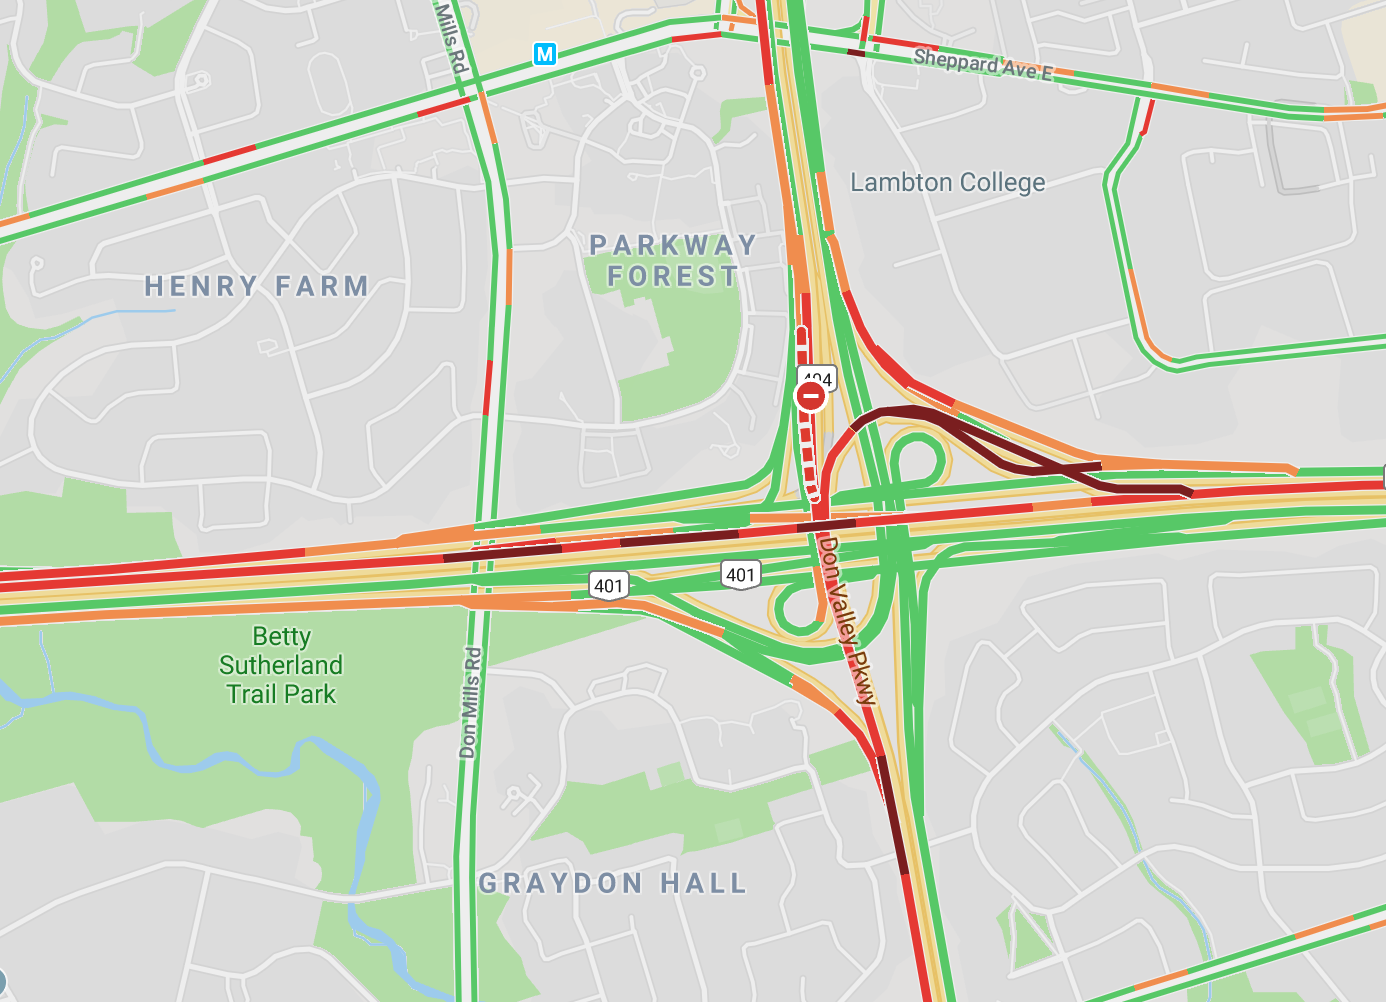
\includegraphics[width=1\linewidth]{graph2.png}
\caption{Toronto's congested roadways}
\end{figure}

\begin{figure}
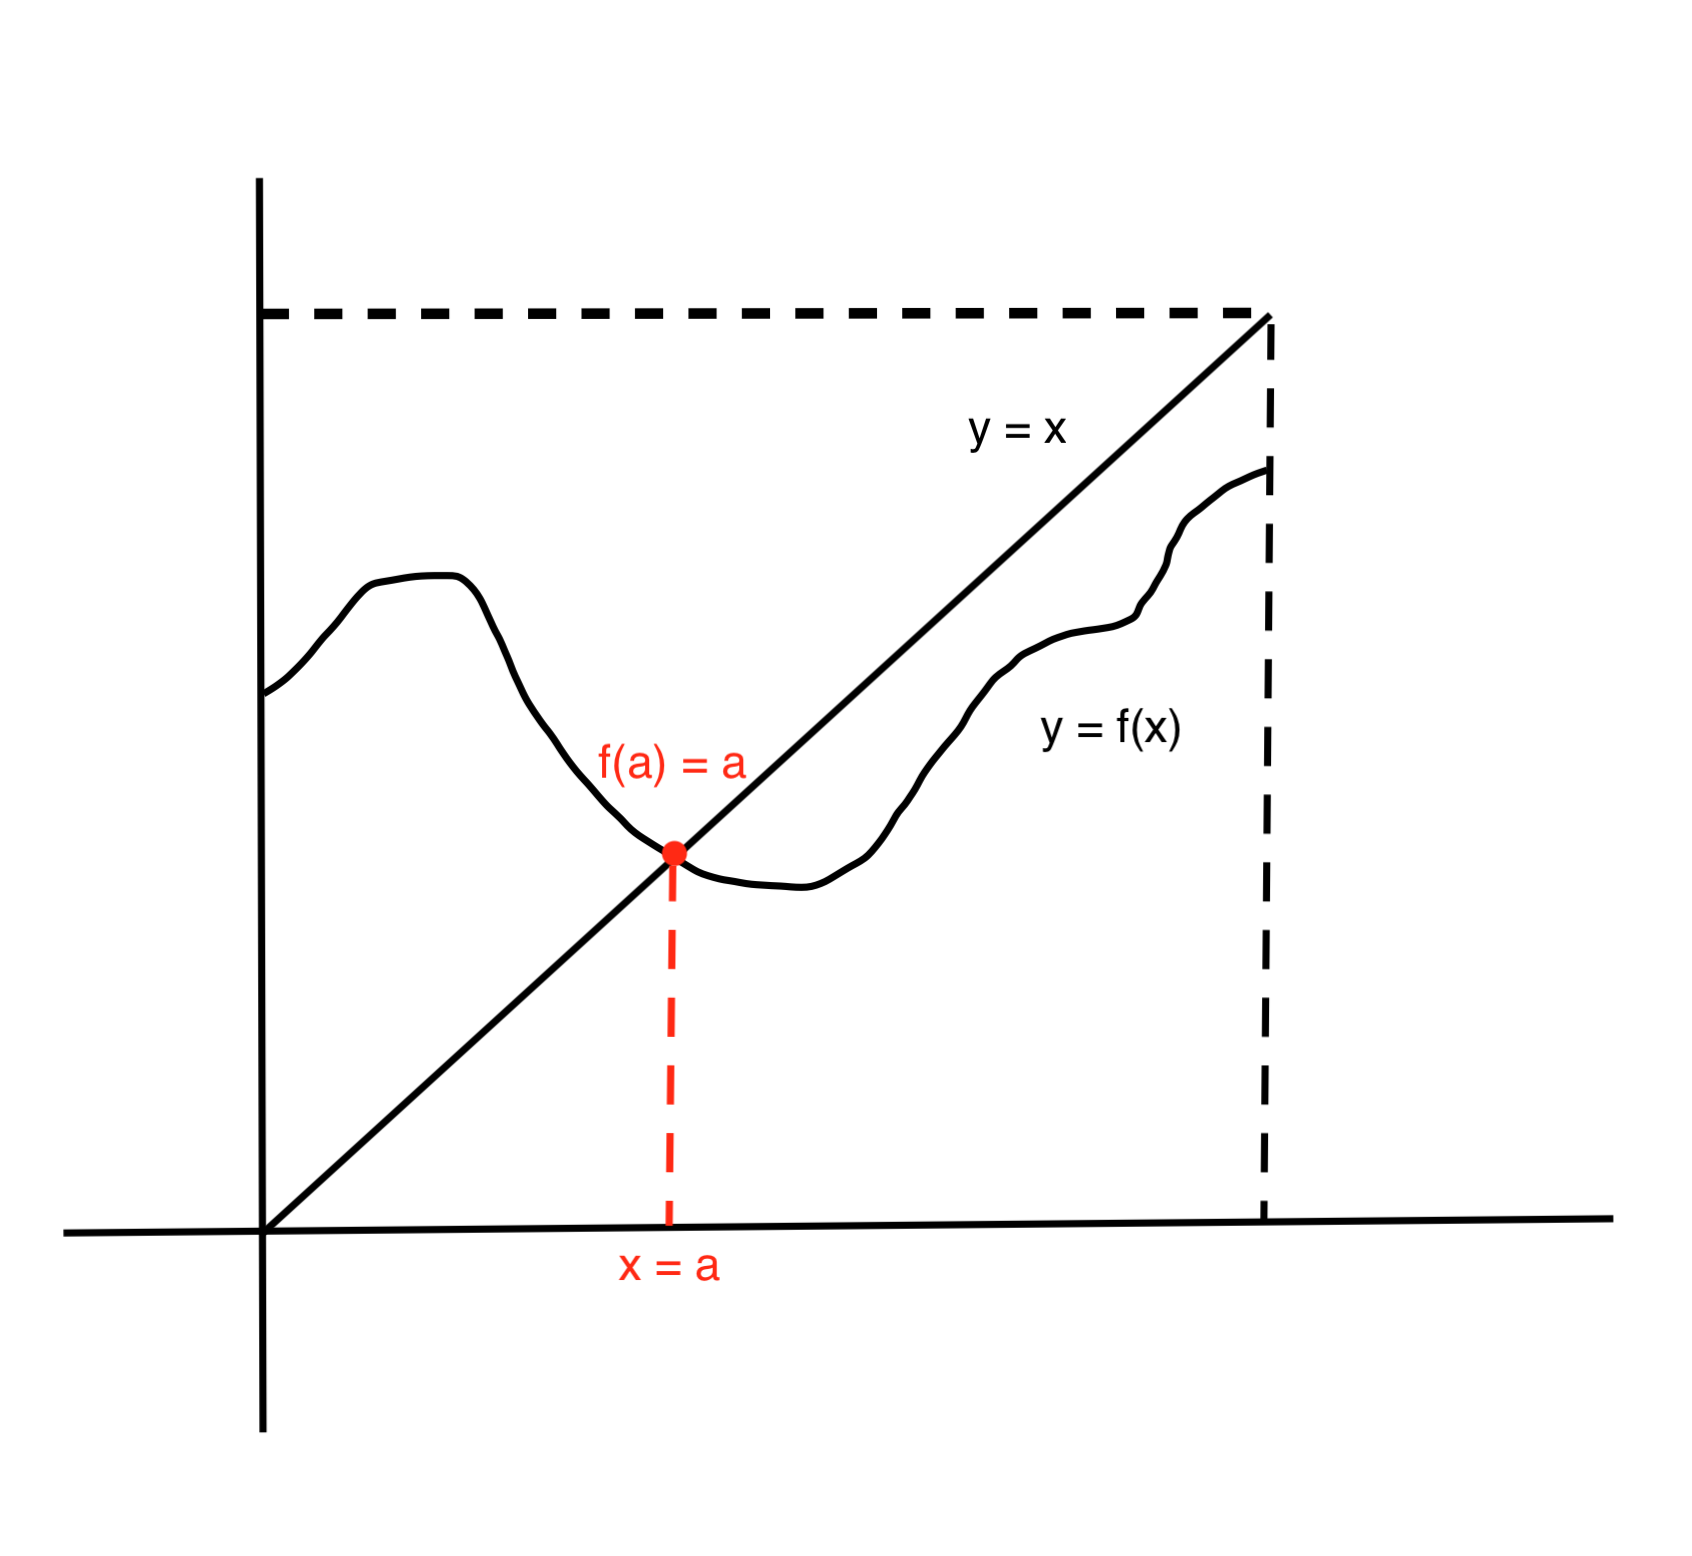
\includegraphics[width=0.9\linewidth]{fixed2.png}
\caption{A graphical representation of BFPT}
\end{figure}

%----------------------------------------------------------------------------------------

\end{column} % End of the first column

\begin{column}{\sepwid}\end{column} % Empty spacer column

\begin{column}{\twocolwid} % Begin a column which is two columns wide (column 2)

\begin{columns}[t, totalwidth=\twocolwid] % Split up the two columns wide column

\begin{column}{\onecolwid}\vspace{-.6in} % The first column within column 2 (column 2.1)

%----------------------------------------------------------------------------------------
%	MATERIALS
%----------------------------------------------------------------------------------------

\begin{block}{Game Theory}

Game theory is the mathematical study of collections of players interacting in a logic fashion, each with the goal of maximizing their personal outcome.
\newline\newline
A game is composed of a set of $n$ players playing the game, a set of possible actions for each player, which we will call $S^i$ for each $i$ from $1$ to $n$, and finally, a payout function, which maps a tuple of strategies from each player's set of strategies to the real numbers, giving a payout value for each player, if a given set of strategies is played. The payout function for the $i$-th player is defined as $f^i: \ S^1 \times S^2 \times ... \times S^n \ \rightarrow \ \mathbb{R}$.
We can extend this definition of a game to define the Nash Equilibrium.

\end{block}

%----------------------------------------------------------------------------------------

\end{column} % End of column 2.1



\begin{column}{\onecolwid}\vspace{-.6in} % The second column within column 2 (column 2.2)

%----------------------------------------------------------------------------------------
%	METHODS
%----------------------------------------------------------------------------------------

% Please add the following required packages to your document preamble:
% \usepackage{multirow}

\begin{figure}
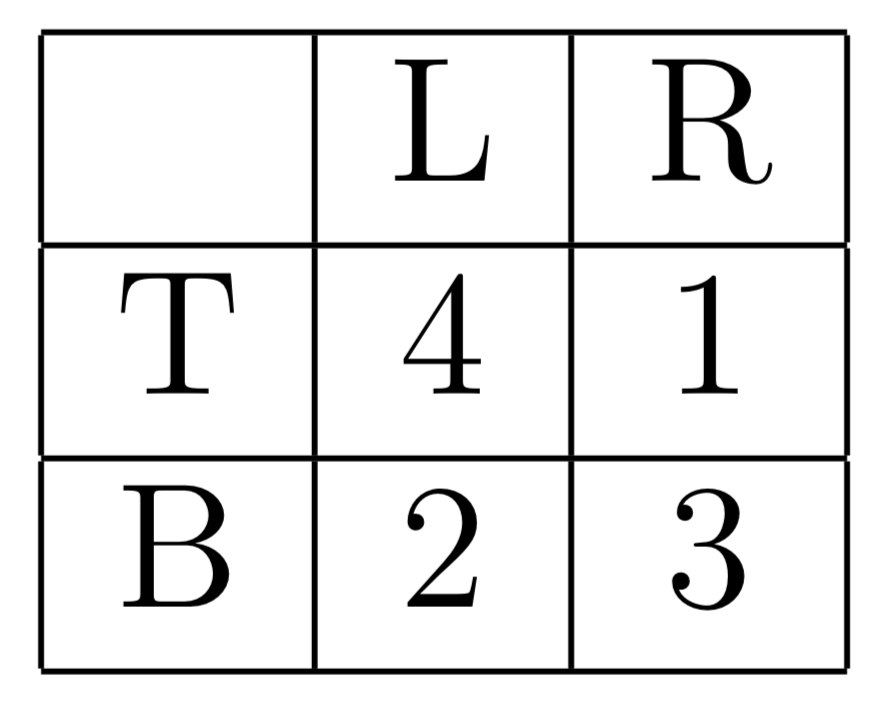
\includegraphics[width=0.4\linewidth]{payout.png}
\caption{A game that does not have a pure strategy Nash Equilibrium}
\end{figure}

{\fontfamily{ComputerModern}\selectfont
A Nash Equilibrium is a set of strategies where no player can change their strategy and get a better outcome. A pure strategy equilibrium is one in which each of the players choose their strategies with certainty. The game above has a \textbf{mixed strategy} equilibrium, in which the players choose their respective strategies probabilistically.
\vspace{10mm}
}




%----------------------------------------------------------------------------------------

\end{column} % End of column 2.2




\end{columns} % End of the split of column 2 - any content after this will now take up 2 columns width


%----------------------------------------------------------------------------------------
%	IMPORTANT RESULT
%----------------------------------------------------------------------------------------

\begin{alertblock}{Nash's Theorem}

For every non-cooperative game with a finite number of players, each with a finite number of strategies, there exists at least one \textbf{Nash Equilibrium}. That is, for a set of $n$ players, there exists a collection of strategies, $(s_1, \ s_2, \ ... \ , \ s_{n-1}, \ s_n)$, such that for the $i$-th player, there exists no different strategy in their personal strategy set, $\hat{s}$, such that $f^i(s_1, \ s_2, \ ... \ , \ s_{n-1}, \ s_n) \ < \ f^i(s_1, \ s_2, \ ... \ , \ s_{i-1}, \ \hat{s}, \ s_{i+1}, \ ... \ , \ s_{n-1}, \ s_n)$.

\end{alertblock} 

%----------------------------------------------------------------------------------------

\begin{columns}[t,totalwidth=\twocolwid] % Split up the two columns wide column again

\begin{column}{\onecolwid} % The first column within column 2 (column 2.1)

%----------------------------------------------------------------------------------------
%	MATHEMATICAL SECTION
%----------------------------------------------------------------------------------------

\begin{block}{Brouwer's Fixed Point Theorem}

Brouwer's Fixed Point Theorem (BFPT) states that if $f : D^{n} \rightarrow D^{n}$ is continuous from the $n$-disk to itself, then the mapping $f$ has a fixed point (formally, a point $x^{*}$, such that $f(x^{*}) = x^{*}$). \newline 

BFPT is significant because it can be used to prove Nash's Theorem. Conceptually, if we define a function that, for a set of strategies, maps the current strategy to a more optimal strategy (one that has a better payout value for some player), then by BFPT, this function must have a fixed point. This means that there must be a set of strategies such that this strategy set is mapped to itself, demonstrating that no strategy set that is more optimal can be achieved (a Nash Equilibrium). The rigorous proof of this concept requires much more nuance and definitions. In order to prove BFPT, a construction known as Sperner's Lemma can be utilized.



\end{block}

%----------------------------------------------------------------------------------------

\end{column} % End of column 2.1

\begin{column}{\onecolwid} % The second column within column 2 (column 2.2)

%----------------------------------------------------------------------------------------
%	RESULTS
%----------------------------------------------------------------------------------------

\begin{block}{Sperner's Lemma}

\begin{figure}
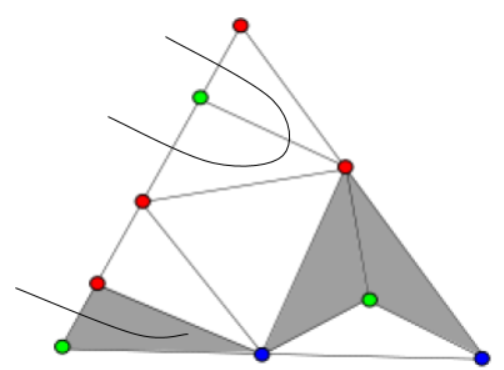
\includegraphics[width=0.8\linewidth]{Capture1.PNG}
\caption{Sperner labeling of a triangle}
\end{figure}

Let $\tau$ be a Sperner triangulation. Then there exists a triangle in $\tau$ labelled red, green, blue. We can prove this by demonstrating that there must exist a path through the triangle that terminates in a triangulation with a red, blue, green labeling.


\end{block}

%----------------------------------------------------------------------------------------

\end{column} % End of column 2.2

\end{columns} % End of the split of column 2

\end{column} % End of the second column

\begin{column}{\sepwid}\end{column} % Empty spacer column

\begin{column}{\onecolwid} % The third column

%----------------------------------------------------------------------------------------
%	CONCLUSION
%----------------------------------------------------------------------------------------

\begin{block}{Graph Theory and Modelling}

In order to combine the ideas in game theory with traffic network optimization, a road network can be represented as a graph (a collection of nodes and edges). Each of the edges on the graph has an associated weight, corresponding to the time it takes for a car or a 'player' to drive down the 'road', represented by an edge. By utilizing Dijkstra's Algorithm, a computational model can be created in which the optimal route for each player that enters the road network can be calculated, therefore modelling a system of traffic.

\end{block}

\begin{figure}
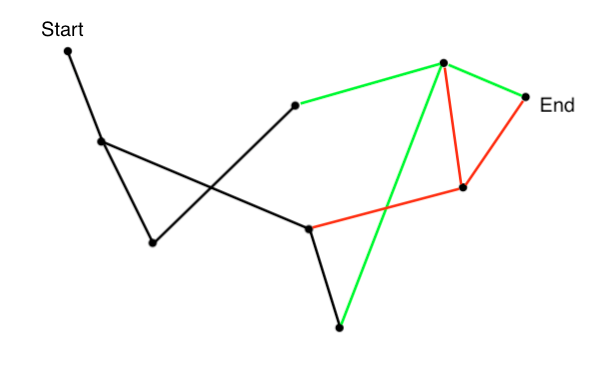
\includegraphics[width=0.8\linewidth]{graph.png}
\caption{Example of a graph representing a road network}
\end{figure}
%----------------------------------------------------------------------------------------
%	ADDITIONAL INFORMATION
%----------------------------------------------------------------------------------------

\begin{block}{Conclusion and Applications}

One way we can relate all of this back to traffic network optimization is through Braess' Paradox. This is a phenomenon where adding a road to a network, represented by a graph, can increase traffic congestion.

\begin{figure}
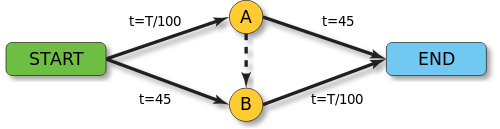
\includegraphics[width=0.8\linewidth]{braess.png}
\caption{A visual representation of Braess' Paradox}
\end{figure}

In order to understand systems like this, we can examine the \textbf{Price of Anarchy}, which is a measurement of the inefficiency of a system due to the selfish nature of the players in it. By finding the Nash Equilibrium, as well as the optimal configuration of the system, where the gain for all players is maximized, we can ultimately better understand how to construct networks such that inefficiency is minimized.




\end{block}


%----------------------------------------------------------------------------------------
%	Image
%----------------------------------------------------------------------------------------

%----------------------------------------------------------------------------------------
%	Image
%----------------------------------------------------------------------------------------



%----------------------------------------------------------------------------------------
%	Image
%----------------------------------------------------------------------------------------



%----------------------------------------------------------------------------------------

\end{column} % End of the third column

\end{columns} % End of all the columns in the poster

\end{frame} % End of the enclosing frame

\end{document}
